\documentclass{ximera}

%\usepackage{todonotes}

\newcommand{\todo}{}

\usepackage{esint} % for \oiint
\ifxake%%https://math.meta.stackexchange.com/questions/9973/how-do-you-render-a-closed-surface-double-integral
\renewcommand{\oiint}{{\large\bigcirc}\kern-1.56em\iint}
\fi


\graphicspath{
  {./}
  {ximeraTutorial/}
  {basicPhilosophy/}
  {functionsOfSeveralVariables/}
  {normalVectors/}
  {lagrangeMultipliers/}
  {vectorFields/}
  {greensTheorem/}
  {shapeOfThingsToCome/}
  {dotProducts/}
  {partialDerivativesAndTheGradientVector/}
  {../productAndQuotientRules/exercises/}
  {../normalVectors/exercisesParametricPlots/}
  {../continuityOfFunctionsOfSeveralVariables/exercises/}
  {../partialDerivativesAndTheGradientVector/exercises/}
  {../directionalDerivativeAndChainRule/exercises/}
  {../commonCoordinates/exercisesCylindricalCoordinates/}
  {../commonCoordinates/exercisesSphericalCoordinates/}
  {../greensTheorem/exercisesCurlAndLineIntegrals/}
  {../greensTheorem/exercisesDivergenceAndLineIntegrals/}
  {../shapeOfThingsToCome/exercisesDivergenceTheorem/}
  {../greensTheorem/}
  {../shapeOfThingsToCome/}
  {../separableDifferentialEquations/exercises/}
  {vectorFields/}
}

\newcommand{\mooculus}{\textsf{\textbf{MOOC}\textnormal{\textsf{ULUS}}}}

\usepackage{tkz-euclide}
\usepackage{tikz}
\usepackage{tikz-cd}
\usetikzlibrary{arrows}
\tikzset{>=stealth,commutative diagrams/.cd,
  arrow style=tikz,diagrams={>=stealth}} %% cool arrow head
\tikzset{shorten <>/.style={ shorten >=#1, shorten <=#1 } } %% allows shorter vectors

\usetikzlibrary{backgrounds} %% for boxes around graphs
\usetikzlibrary{shapes,positioning}  %% Clouds and stars
\usetikzlibrary{matrix} %% for matrix
\usepgfplotslibrary{polar} %% for polar plots
\usepgfplotslibrary{fillbetween} %% to shade area between curves in TikZ
%\usetkzobj{all}
\usepackage[makeroom]{cancel} %% for strike outs
%\usepackage{mathtools} %% for pretty underbrace % Breaks Ximera
%\usepackage{multicol}
\usepackage{pgffor} %% required for integral for loops



%% http://tex.stackexchange.com/questions/66490/drawing-a-tikz-arc-specifying-the-center
%% Draws beach ball
\tikzset{pics/carc/.style args={#1:#2:#3}{code={\draw[pic actions] (#1:#3) arc(#1:#2:#3);}}}



\usepackage{array}
\setlength{\extrarowheight}{+.1cm}
\newdimen\digitwidth
\settowidth\digitwidth{9}
\def\divrule#1#2{
\noalign{\moveright#1\digitwidth
\vbox{\hrule width#2\digitwidth}}}




% \newcommand{\RR}{\mathbb R}
% \newcommand{\R}{\mathbb R}
% \newcommand{\N}{\mathbb N}
% \newcommand{\Z}{\mathbb Z}

\newcommand{\sagemath}{\textsf{SageMath}}


%\renewcommand{\d}{\,d\!}
%\renewcommand{\d}{\mathop{}\!d}
%\newcommand{\dd}[2][]{\frac{\d #1}{\d #2}}
%\newcommand{\pp}[2][]{\frac{\partial #1}{\partial #2}}
% \renewcommand{\l}{\ell}
%\newcommand{\ddx}{\frac{d}{\d x}}

% \newcommand{\zeroOverZero}{\ensuremath{\boldsymbol{\tfrac{0}{0}}}}
%\newcommand{\inftyOverInfty}{\ensuremath{\boldsymbol{\tfrac{\infty}{\infty}}}}
%\newcommand{\zeroOverInfty}{\ensuremath{\boldsymbol{\tfrac{0}{\infty}}}}
%\newcommand{\zeroTimesInfty}{\ensuremath{\small\boldsymbol{0\cdot \infty}}}
%\newcommand{\inftyMinusInfty}{\ensuremath{\small\boldsymbol{\infty - \infty}}}
%\newcommand{\oneToInfty}{\ensuremath{\boldsymbol{1^\infty}}}
%\newcommand{\zeroToZero}{\ensuremath{\boldsymbol{0^0}}}
%\newcommand{\inftyToZero}{\ensuremath{\boldsymbol{\infty^0}}}



% \newcommand{\numOverZero}{\ensuremath{\boldsymbol{\tfrac{\#}{0}}}}
% \newcommand{\dfn}{\textbf}
% \newcommand{\unit}{\,\mathrm}
% \newcommand{\unit}{\mathop{}\!\mathrm}
% \newcommand{\eval}[1]{\bigg[ #1 \bigg]}
% \newcommand{\seq}[1]{\left( #1 \right)}
% \renewcommand{\epsilon}{\varepsilon}
% \renewcommand{\phi}{\varphi}


% \renewcommand{\iff}{\Leftrightarrow}

% \DeclareMathOperator{\arccot}{arccot}
% \DeclareMathOperator{\arcsec}{arcsec}
% \DeclareMathOperator{\arccsc}{arccsc}
% \DeclareMathOperator{\si}{Si}
% \DeclareMathOperator{\scal}{scal}
% \DeclareMathOperator{\sign}{sign}


%% \newcommand{\tightoverset}[2]{% for arrow vec
%%   \mathop{#2}\limits^{\vbox to -.5ex{\kern-0.75ex\hbox{$#1$}\vss}}}
% \newcommand{\arrowvec}[1]{{\overset{\rightharpoonup}{#1}}}
% \renewcommand{\vec}[1]{\arrowvec{\mathbf{#1}}}
% \renewcommand{\vec}[1]{{\overset{\boldsymbol{\rightharpoonup}}{\mathbf{#1}}}}

% \newcommand{\point}[1]{\left(#1\right)} %this allows \vector{ to be changed to \vector{ with a quick find and replace
% \newcommand{\pt}[1]{\mathbf{#1}} %this allows \vec{ to be changed to \vec{ with a quick find and replace
% \newcommand{\Lim}[2]{\lim_{\point{#1} \to \point{#2}}} %Bart, I changed this to point since I want to use it.  It runs through both of the exercise and exerciseE files in limits section, which is why it was in each document to start with.

% \DeclareMathOperator{\proj}{\mathbf{proj}}
% \newcommand{\veci}{{\boldsymbol{\hat{\imath}}}}
% \newcommand{\vecj}{{\boldsymbol{\hat{\jmath}}}}
% \newcommand{\veck}{{\boldsymbol{\hat{k}}}}
% \newcommand{\vecl}{\vec{\boldsymbol{\l}}}
% \newcommand{\uvec}[1]{\mathbf{\hat{#1}}}
% \newcommand{\utan}{\mathbf{\hat{t}}}
% \newcommand{\unormal}{\mathbf{\hat{n}}}
% \newcommand{\ubinormal}{\mathbf{\hat{b}}}

% \newcommand{\dotp}{\bullet}
% \newcommand{\cross}{\boldsymbol\times}
% \newcommand{\grad}{\boldsymbol\nabla}
% \newcommand{\divergence}{\grad\dotp}
% \newcommand{\curl}{\grad\cross}
%\DeclareMathOperator{\divergence}{divergence}
%\DeclareMathOperator{\curl}[1]{\grad\cross #1}
% \newcommand{\lto}{\mathop{\longrightarrow\,}\limits}

% \renewcommand{\bar}{\overline}

\colorlet{textColor}{black}
\colorlet{background}{white}
\colorlet{penColor}{blue!50!black} % Color of a curve in a plot
\colorlet{penColor2}{red!50!black}% Color of a curve in a plot
\colorlet{penColor3}{red!50!blue} % Color of a curve in a plot
\colorlet{penColor4}{green!50!black} % Color of a curve in a plot
\colorlet{penColor5}{orange!80!black} % Color of a curve in a plot
\colorlet{penColor6}{yellow!70!black} % Color of a curve in a plot
\colorlet{fill1}{penColor!20} % Color of fill in a plot
\colorlet{fill2}{penColor2!20} % Color of fill in a plot
\colorlet{fillp}{fill1} % Color of positive area
\colorlet{filln}{penColor2!20} % Color of negative area
\colorlet{fill3}{penColor3!20} % Fill
\colorlet{fill4}{penColor4!20} % Fill
\colorlet{fill5}{penColor5!20} % Fill
\colorlet{gridColor}{gray!50} % Color of grid in a plot

\newcommand{\surfaceColor}{violet}
\newcommand{\surfaceColorTwo}{redyellow}
\newcommand{\sliceColor}{greenyellow}




\pgfmathdeclarefunction{gauss}{2}{% gives gaussian
  \pgfmathparse{1/(#2*sqrt(2*pi))*exp(-((x-#1)^2)/(2*#2^2))}%
}


%%%%%%%%%%%%%
%% Vectors
%%%%%%%%%%%%%

%% Simple horiz vectors
\renewcommand{\vector}[1]{\left\langle #1\right\rangle}


%% %% Complex Horiz Vectors with angle brackets
%% \makeatletter
%% \renewcommand{\vector}[2][ , ]{\left\langle%
%%   \def\nextitem{\def\nextitem{#1}}%
%%   \@for \el:=#2\do{\nextitem\el}\right\rangle%
%% }
%% \makeatother

%% %% Vertical Vectors
%% \def\vector#1{\begin{bmatrix}\vecListA#1,,\end{bmatrix}}
%% \def\vecListA#1,{\if,#1,\else #1\cr \expandafter \vecListA \fi}

%%%%%%%%%%%%%
%% End of vectors
%%%%%%%%%%%%%

%\newcommand{\fullwidth}{}
%\newcommand{\normalwidth}{}



%% makes a snazzy t-chart for evaluating functions
%\newenvironment{tchart}{\rowcolors{2}{}{background!90!textColor}\array}{\endarray}

%%This is to help with formatting on future title pages.
\newenvironment{sectionOutcomes}{}{}



%% Flowchart stuff
%\tikzstyle{startstop} = [rectangle, rounded corners, minimum width=3cm, minimum height=1cm,text centered, draw=black]
%\tikzstyle{question} = [rectangle, minimum width=3cm, minimum height=1cm, text centered, draw=black]
%\tikzstyle{decision} = [trapezium, trapezium left angle=70, trapezium right angle=110, minimum width=3cm, minimum height=1cm, text centered, draw=black]
%\tikzstyle{question} = [rectangle, rounded corners, minimum width=3cm, minimum height=1cm,text centered, draw=black]
%\tikzstyle{process} = [rectangle, minimum width=3cm, minimum height=1cm, text centered, draw=black]
%\tikzstyle{decision} = [trapezium, trapezium left angle=70, trapezium right angle=110, minimum width=3cm, minimum height=1cm, text centered, draw=black]


\title{Describe Everything}

\begin{document}

\begin{abstract}
features
\end{abstract}
\maketitle







\begin{example} Analyze


Completely analyze $K(w) = w \sqrt{9-w}$ with   $K'(w) = \sqrt{9 - w} + w \frac{1}{2} (9 - w)^{-\tfrac{1}{2}} (-1)$


$K$ is not an elementary function.  It is the product of a linear function and a root function.


\textbf{Domain}



The domian of $K$ consists of the real numbers that are included in both domains of both factor functions.


$w$ is a linear function, so its domain is $(-\infty, \infty)$.



$\sqrt{9-w}$ is a root function.  The inside must be nonnegative. The decide this, we first find the zero of $9 - w$, which is $9$. \\

Since $9 - w$ is a linear function with a negative leading coefficient, $9 - w > 0$ on $(-\infty, 9)$.

Therefore, ther domain of $K$ is $(-\infty, 9]$. \\




\textbf{Zeros}

$K$ is already written in factored form, so we will use the zero product property.


Either $w = 0$ or $\sqrt{9-w} = 0$. \\

Either $w = 0$ or $w = 9$. \\


$K$ has two zeros, $0$ and $9$. \\




\textbf{Continuity}

LInear and root functions are both continuous, so is there product.






\textbf{End-Behavior}


We only have one direction for end-behavior. \\


Since $w$ is a linear function with a positive leading coefficient, we know that 
$\lim\limits_{w \to -\infty} w = -\infty$.  It is unbounded negatively. \\

Since $\sqrt{9-w}$ is a root funciton with a positive leading coefficient, we know that $\lim\limits_{w \to -\infty} \sqrt{9-w} = \infty$.   It is unbounded negatively. \\


The product of two functions which are both unbounded is unbounded.  Since one takes on negative values and the ohter postive values, their product is negative.


\[
\lim\limits_{w \to -\infty} K(w) = -\infty
\]




\textbf{Behavior (Increasing and Decreasing)}


We'll use the derivative.



\[
K'(w) = \sqrt{9 - w} + w \frac{1}{2} (9 - w)^{-\tfrac{1}{2}} (-1)
\]


\[
=   \frac{1}{2 \sqrt{9-w}} \, (2(9-w) - w) 
\]


\[
=   \frac{1}{2 \sqrt{9-w}} \, (18 - 3w) 
\]


\[
=   \frac{3}{2 \sqrt{9-w}} \, (6 - w) 
\]


$6$ is a domain number and a zero of the derivative.  That makes $6$ a critical number. \\


$9$ is a domain number where the derivative does not exist.  That makes $9$ a critical number. \\



$K'(w)$ is a product.  The root factor is always positive, so the sign of $K'(w)$ is the same as the sign of $6 - w$. \\


$6 - w$ is a linear function with a negative leading coeffcient. So, $6 - w > 0$ on $(-\infty, 6)$ and $6 - w < 0$ on $(6, 9)$.



$\blacktriangleright$ $K$ is increasing on $(-\infty, 6)$ \\

$\blacktriangleright$ $K$ is decreasing on $(6, 9)$ \\





\textbf{Global Maximum and Minimum)}



Since $\lim\limits_{w \to -\infty} K(w) = -\infty$, there is no global minimum. \\


Since $K$ is increasing on $(-\infty, 6)$ and $K$ is decreasing on $(6, 9)$, $K$ has a global maximum at $6$.  \\

The global maximum value is $K(6) = 6 \sqrt{9 - 6} = 6 \sqrt{3}$. \\




\textbf{Local Maximum and Minimum)}


Since global maximums are automatically local maximums, $6 \sqrt{3}$ is a local maximum. \\


We also have the critical number $9$ with $K(9) = 0$.  This is a local minimum.  We can see this because $K$ is contiuous and decreasing on the interval $(6, 9]$. \\









\textbf{Range)}

\begin{itemize}
  \item $K$ is continuous
  \item $6 \sqrt{3}$ is the global maximum
  \item $\lim\limits_{w \to -\infty} K(w) = -\infty$
\end{itemize}

That gives a range of $(-\infty, 6 \sqrt{3}]$.




This all agrees with the graph. \\




\textbf{\textcolor{blue!55!black}{$\blacktriangleright$ desmos graph}} 
\begin{center}
\desmos{9y96v7ef1w}{400}{300}
\end{center}






\end{example}


































We do have alternatives to the derivative for some types of functions. \\







\begin{procedure} Critical Number


Earlier in the course, we saw an algebraic method of identifying the critical number in the previous example.  We can apply the same method here.


We think there is a hump in the graph of $K$ and at the highest point, $(A, A\sqrt{9-A})$, the tangent line would be horizontal.



\begin{image}
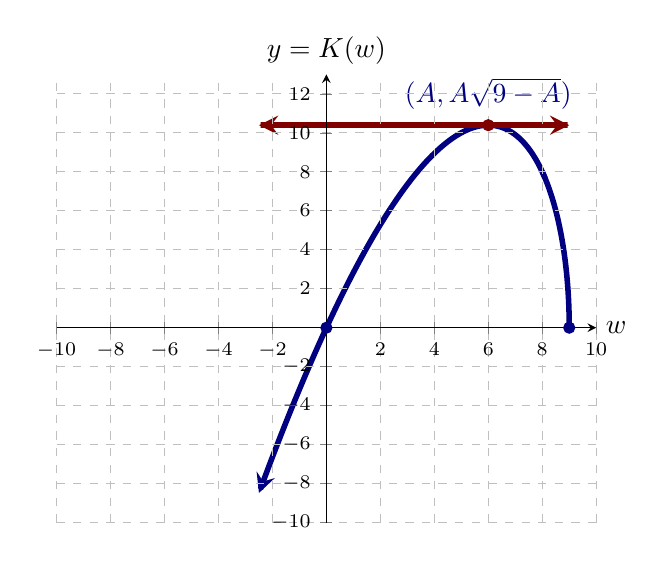
\begin{tikzpicture}
  \begin{axis}[
            domain=-10:10, ymax=13, xmax=10, ymin=-10, xmin=-10,
            axis lines =center, xlabel=$w$, ylabel={$y=K(w)$}, grid = major, grid style={dashed},
            ytick={-10,-8,-6,-4,-2,2,4,6,8,10,12},
            xtick={-10,-8,-6,-4,-2,2,4,6,8,10},
            yticklabels={$-10$,$-8$,$-6$,$-4$,$-2$,$2$,$4$,$6$,$8$,$10$,$12$}, 
            xticklabels={$-10$,$-8$,$-6$,$-4$,$-2$,$2$,$4$,$6$,$8$,$10$},
            ticklabel style={font=\scriptsize},
            every axis y label/.style={at=(current axis.above origin),anchor=south},
            every axis x label/.style={at=(current axis.right of origin),anchor=west},
            axis on top
          ]


          \addplot [line width=2, penColor, smooth,samples=200,domain=(-2.5:8.1),<-] {x * sqrt(9-x)};
          \addplot [line width=2, penColor, smooth,samples=300,domain=(8:9)] {x * sqrt(9-x)};
          \addplot [line width=2, penColor2, smooth,samples=200,domain=(-2.5:9),<->] {10.39};
         


          \addplot[color=penColor,fill=penColor,only marks,mark=*] coordinates{(0,0)};
          \addplot[color=penColor,fill=penColor,only marks,mark=*] coordinates{(9,0)};
          \addplot[color=penColor2,fill=penColor2,only marks,mark=*] coordinates{(6,10.39)};


          \node at (axis cs:6,12) [penColor] {$(A, A\sqrt{9-A})$};


           

  \end{axis}
\end{tikzpicture}
\end{image}


Now, create a new function called $F$.

\[
F(x) = K(x) - K(A) = K(x) - A\sqrt{9-A}
\]


As we saw earlier, since we have a tangent line, the difference of the original function and the linear function has a double root at $A$.  $x-A$ divides evenly into $F$.  And, the resulting function then also has $A$ as a root.  

First, factor out $x-A$ from $F$.


\[
x\sqrt{9-x} - A\sqrt{9-A} = \frac{x\sqrt{9-x} - A\sqrt{9-A}}{1} \cdot \frac{x\sqrt{9-x} + A\sqrt{9-A}}{\answer{x\sqrt{9-x} + A\sqrt{9-A}}}
\]

\[
= \frac{x^2 (9-x) - A^2 (9-A)}{x\sqrt{9-x} + A\sqrt{9-A}} = \frac{9x^2 - x^3 - 9A^2 + A^3}{x\sqrt{9-x} + A\sqrt{9-A}}
\]


\[
= \frac{9(x^2-A^2) - (x^3 - A^3)}{x\sqrt{9-x} + A\sqrt{9-A}} = \frac{(x-A)(9(x+A)-(x^2 + xA + A^2))}{x\sqrt{9-x} + A\sqrt{9-A}}
\]


$x-A$ divides into this evenly leaving

\[
\frac{9(x+A)-(x^2 + xA + A^2)}{x\sqrt{9-x} + A\sqrt{9-A}}
\]

$A$ is a root of this, which means $A$ is a root of the numerator.


\[
9(A+A)-(A^2 + A^2 + A^2) = 0
\]

\[
18A - 3A^2 = 0
\]

\[
3A \left(\answer{6-A} \right) = 0
\]


The zero we are looking for is $6$.
The critical number is $6$ and $K(6) = 6 \sqrt{3}$.


\end{procedure}




















\begin{center}
\textbf{\textcolor{green!50!black}{ooooo-=-=-=-ooOoo-=-=-=-ooooo}} \\

more examples can be found by following this link\\ \link[More Examples of Function Analysis]{https://ximera.osu.edu/csccmathematics/precalculus1/precalculus1/functionAnalysis/examples/exampleList}

\end{center}




\end{document}
